\documentclass[12pt,letterpaper]{article}
\usepackage[utf8]{inputenc}
\usepackage{tikz}
\usetikzlibrary{trees}
\usepackage[spanish, es-nodecimaldot]{babel}
\usepackage{amsmath}
\usepackage{color}
\usepackage{algorithm}
\usepackage[noend]{algpseudocode}
\renewcommand{\algorithmicrequire}{\textbf{Entrada:}}
\renewcommand{\algorithmicensure}{\textbf{Salida:}}
\usepackage{subcaption}
\usepackage{amsfonts}
\usepackage{hyperref}
 \hypersetup{
     colorlinks=true,
     linkcolor=blue,
     filecolor=blue,
     citecolor = blue,      
     urlcolor=cyan,
     }
\usepackage{amssymb}
\usepackage{listings}
\usepackage{color}

\definecolor{mygreen}{rgb}{0,0.6,0}
\definecolor{mygray}{rgb}{0.5,0.5,0.5}
\definecolor{mymauve}{rgb}{0.58,0,0.82}

\lstset{ 
  backgroundcolor=\color{white},   % choose the background color; you must add \usepackage{color} or \usepackage{xcolor}; should come as last argument
  basicstyle=\footnotesize,        % the size of the fonts that are used for the code
  breakatwhitespace=false,         % sets if automatic breaks should only happen at whitespace
  breaklines=true,                 % sets automatic line breaking
  captionpos=b,                    % sets the caption-position to bottom
  commentstyle=\color{mygreen},    % comment style
  deletekeywords={...},            % if you want to delete keywords from the given language
  escapeinside={\%*}{*)},          % if you want to add LaTeX within your code
  extendedchars=true,              % lets you use non-ASCII characters; for 8-bits encodings only, does not work with UTF-8
  firstnumber=1,                % start line enumeration with line 1000
  frame=single,	                   % adds a frame around the code
  keepspaces=true,                 % keeps spaces in text, useful for keeping indentation of code (possibly needs columns=flexible)
  keywordstyle=\color{blue},       % keyword style
  language=Octave,                 % the language of the code
  morekeywords={*,...},            % if you want to add more keywords to the set
  numbers=none,                    % where to put the line-numbers; possible values are (none, left, right)
  numbersep=5pt,                   % how far the line-numbers are from the code
  numberstyle=\tiny\color{mygray}, % the style that is used for the line-numbers
  rulecolor=\color{black},         % if not set, the frame-color may be changed on line-breaks within not-black text (e.g. comments (green here))
  showspaces=false,                % show spaces everywhere adding particular underscores; it overrides 'showstringspaces'
  showstringspaces=false,          % underline spaces within strings only
  showtabs=false,                  % show tabs within strings adding particular underscores
  stepnumber=2,                    % the step between two line-numbers. If it's 1, each line will be numbered
  stringstyle=\color{mymauve},     % string literal style
  tabsize=2,	                   % sets default tabsize to 2 spaces
  title=\lstname                   % show the filename of files included with \lstinputlisting; also try caption instead of title
}

\usepackage{amsthm}
\newtheorem{theorem}{Teorema}

\usepackage{graphicx}
\usepackage[inner=1.5 cm, outer = 1.5 cm, top=1 cm, bottom = 1.5 cm]{geometry}
\setlength{\parskip}{3mm}
\title{\textsc{Práctica 12: Red neuronal}}
\author{\textsc{Fabiola Vázquez}}
\renewcommand{\lstlistingname}{Código}
\setlength{\parindent}{0cm}

\begin{document}
\maketitle

\hrule
\section{Introducción}
En esta práctica \cite{elisapractica12} se trabaja con el aprendizaje de máquina.  la cuál va a reconocer dígitos que provienen de imágenes pequeñas en blanco y negro. El objetivo es estudiar el desempeño de la red neuronal en términos de su puntaje F en función de las probabilidades asignadas para la generación de los dígitos. El experimento se lleva a cabo en el software R \cite{R} en un cuaderno de Jupyter \cite{jupyter}.

\section{Experimento}
A la máquina se le provee de imágenes que contiene la representación en blanco y negro de algún dígito, la máquina retorna que dígito es. Se lleva el registro de las veces que la máquina acertó en un \texttt{data.frame} y se calculan los totales. El cuadro \ref{dataframe} muestra un ejemplo de dicho \texttt{data.frame}.
Se varía la probabilidad del color negro en $\{0.9925, 0.995, 0.9975\}$, la del color gris en $\{0.9, 0.925, 0.95\}$ y la probabilidad del blanco en $\{0.001, 0.002, 0.003\}$. Para cada combinación de las probabilidades se realizan 50 repeticiones.

Se calcula el puntaje F \cite{F} como
\begin{equation}
\text{F} = 2 \cdot \frac{\text{precisión}\cdot \text{exhaustividad}}{\text{precisión} + \text{exhaustividad}},
\end{equation}
para cada uno de los dígitos con los que se trabaja y al final se calcula la media de los puntajes F. Los resultados se almacenan en un \texttt{data.frame}, el cuadro \ref{data} muestra un fragmento de los datos recopilados.

En la figura \ref{im} se tienen gráficos de caja de las 27 combinaciones, donde el color de la caja representa la probabilidad del color gris, el color del borde representa la probabilidad del color negro y en el eje horizontal está representada la probabilidad del color blanco. 

Se realizan pruebas de correlación para cada una de las probabilidades, obteniendo valores $p$ menores que 0.05, por lo que se concluye que las tres probabilidades afectan al puntaje F. Cuando las probabilidades de los colores negro y gris aumenta, el puntaje F también. Cuando la probabilidad de blanco aumenta, el puntaje F disminuye.
\begin{table}
\centering
\caption{Ejemplo del \texttt{data.frame} recopilado en una corrida }
\begin{tabular}{rrrrrrrrrrrrr}
  \hline
 & 0 & 1 & 2 & 3 & 4 & 5 & 6 & 7 & 8 & 9 & NA & Total \\ 
  \hline
0 & 20 & 0 & 0 & 0 & 0 & 0 & 0 & 0 & 2 & 0 & 0 & 22 \\ 
  1 & 0 & 28 & 0 & 0 & 0 & 0 & 0 & 0 & 0 & 0 & 0 & 28 \\ 
  2 & 0 & 0 & 21 & 0 & 0 & 0 & 0 & 0 & 1 & 0 & 2 & 24 \\ 
  3 & 0 & 0 & 0 & 33 & 0 & 0 & 0 & 0 & 0 & 2 & 1 & 36 \\ 
  4 & 0 & 0 & 0 & 0 & 27 & 2 & 0 & 0 & 0 & 0 & 0 & 29 \\ 
  5 & 0 & 2 & 0 & 1 & 0 & 35 & 0 & 2 & 0 & 0 & 1 & 41 \\ 
  6 & 0 & 0 & 0 & 0 & 5 & 0 & 24 & 0 & 0 & 0 & 1 & 30 \\ 
  7 & 0 & 0 & 0 & 0 & 0 & 0 & 0 & 20 & 0 & 0 & 0 & 20 \\ 
  8 & 1 & 0 & 0 & 0 & 0 & 0 & 1 & 0 & 30 & 0 & 0 & 32 \\ 
  9 & 0 & 1 & 0 & 1 & 0 & 1 & 0 & 0 & 1 & 34 & 0 & 38 \\ 
  Total & 21 & 31 & 21 & 35 & 32 & 38 & 25 & 22 & 34 & 36 & 5 & 300 \\ 
   \hline
\end{tabular}
\label{dataframe}
\end{table}

 \begin{figure}
 	\centering 
		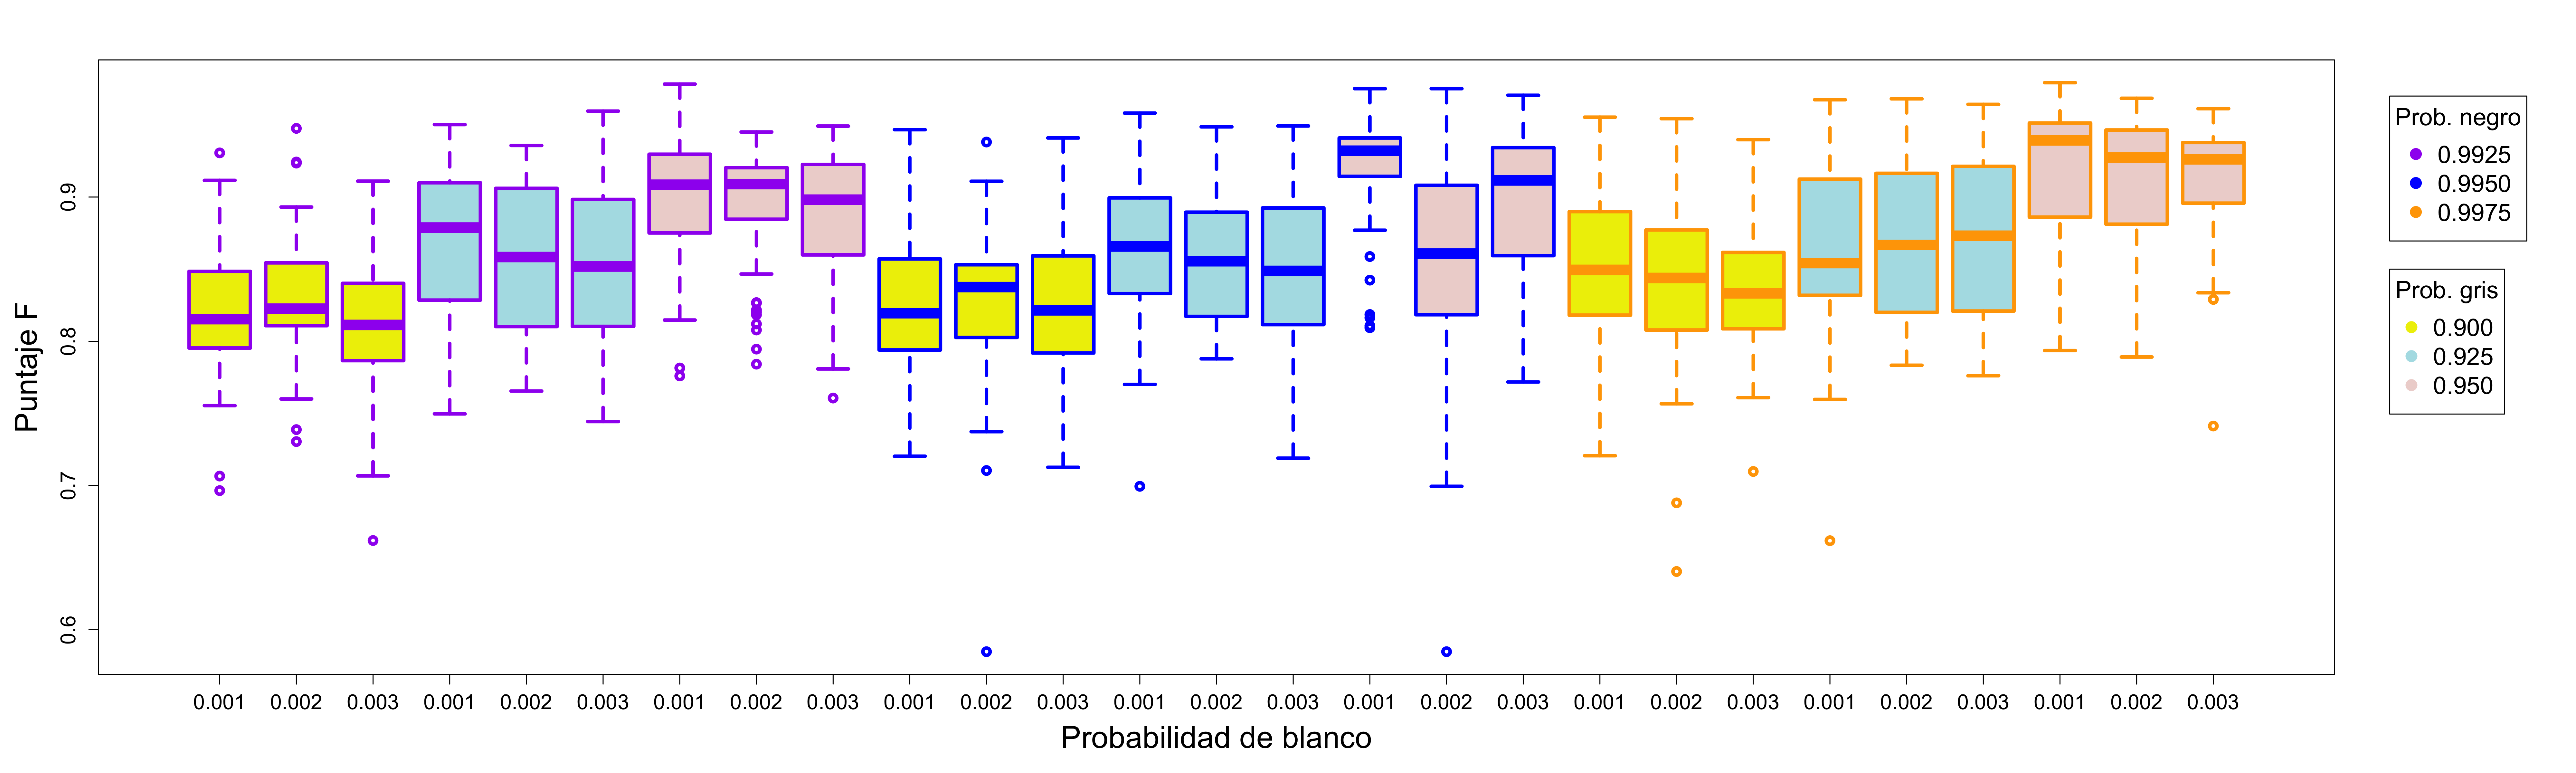
\includegraphics[width=\linewidth]{boxplot.png} 		
		\caption{Gráficos de caja del puntaje F de las diferentes combinaciones.}
		 		\label{im}
 	\end{figure}  




\begin{table}
\centering
\caption{Fragmento de los datos.}
\begin{tabular}{rrrr}
  \hline
Negro & Gris & Blanco & Puntaje F \\ 
  \hline
0.9925 & 0.900 & 0.001 & 0.8345\\
0.9925 & 0.925 & 0.002 & 0.7735\\
0.9950 & 0.950 & 0.002 & 0.9191\\
0.9950 & 0.950 & 0.003 & 0.9657\\
0.9975 & 0.900 & 0.002 & 0.9476\\
0.9975 & 0.950 & 0.002 & 0.9282\\
\hline
\end{tabular}
\label{data}
\end{table}




\bibliographystyle{plain} 
\bibliography{Referencias}


\end{document} 